\documentclass[12pt, a4]{article}
\usepackage[english]{babel}
\usepackage[utf8x]{inputenc}
\usepackage{fullpage}
\usepackage{listings}
\usepackage{graphicx}
\usepackage{color}

%Syntax highlighting
\definecolor{blue-violet}{rgb}{0.54, 0.17, 0.89}
\definecolor{ao}{rgb}{0.0, 0.5, 0.0}
\definecolor{amaranth}{rgb}{0.9, 0.17, 0.31}
\definecolor{ballblue}{rgb}{0.13, 0.67, 0.8}
\definecolor{onyx}{rgb}{0.06, 0.06, 0.06}


\lstset{
  breaklines=true,                 % automatic line breaking only at whitespace
  captionpos=b,                    % sets the caption-position to bottom
  breakatwhitespace=false,
  keepspaces=true,
  numbers=left,
  numbersep=5pt,
  showspaces=false,
  showstringspaces=false,
  showtabs=false,
  tabsize=4,  
  backgroundcolor=\color{white},   % choose the background color
  commentstyle=\color{ao},    % comment style
  keywordstyle=\color{amaranth},    % keyword style
  stringstyle=\color{blue-violet},    % string literal style
  numberstyle=\tiny\color{ballblue},	   % number style
  basicstyle=\ttfamily\footnotesize\color{onyx} % size of fonts used for the code
}

%Document Header
\title{\textbf{Department of CSE\\SSN College of Engineering}}
\author{\textbf{Vishakan Subramanian - 18 5001 196 - Semester VI}}
\date{26 February 2021}

\begin{document}
\maketitle
\hrule
\section*{\center{UCS 1602 - Compiler Design}}
\hrule
\bigskip

%Assignment Details
\subsection*{\center{\textbf{Exercise 4: Recursive Descent Parser Using C}}}
\subsection*{\flushleft{Aim:}}
\begin{flushleft}
Write a program in C to construct \textbf{Recursive Descent Parser} for the following grammar which is for arithmetic expression involving + and *. Check the Grammar for left recursion and convert into suitable for this parser. Write recursive functions for every non-terminal. Call the function for start symbol of the Grammar in main().
\\
G1: \\
\hspace{10mm} E $\rightarrow$ E $+$ T $|$ T \\
\hspace{10mm} T $\rightarrow$ T $*$ F $|$ F \\
\hspace{10mm} F $\rightarrow$ i \\

Extend this parser to include division, subtraction and parenthesis operators.

G2: \\
\hspace{10mm} E $\rightarrow$ E $+$ T $|$ E $-$ T $|$ T \\
\hspace{10mm} T $\rightarrow$ T $*$ F $|$ T $/$ F $|$ F \\
\hspace{10mm} F $\rightarrow$ (E) $|$ i \\
\end{flushleft}

%Code
\newpage
\subsection*{\flushleft{Code - Grammar 1:}}
\begin{flushleft}
\lstinputlisting[language = C]{RDP1.c}
\end{flushleft}

%Output
\newpage
\subsection*{\flushleft{Output - Grammar 1:}}
\begin{figure}[h]
\centering
\caption{Console Output for parsed strings of Grammar 1.}
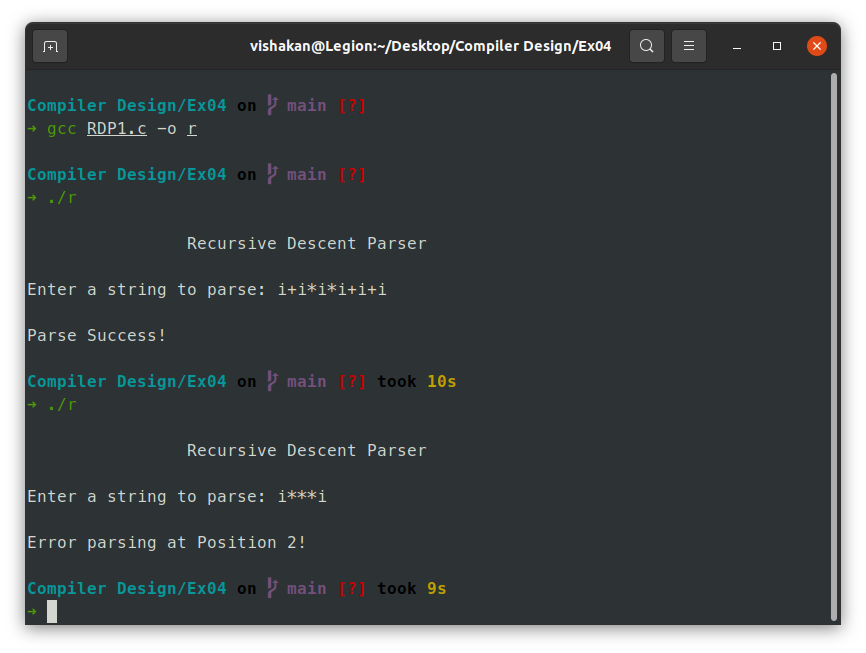
\includegraphics[scale= 0.5]{RDP1OP.png}
\end{figure}

%Code
\newpage
\subsection*{\flushleft{Code - Grammar 2:}}
\begin{flushleft}
\lstinputlisting[language = C]{RDP2.c}
\end{flushleft}

%Output
\newpage
\subsection*{\flushleft{Output - Grammar 2:}}
\begin{figure}[h]
\centering
\caption{Console Output for parsed strings of Grammar 2.}
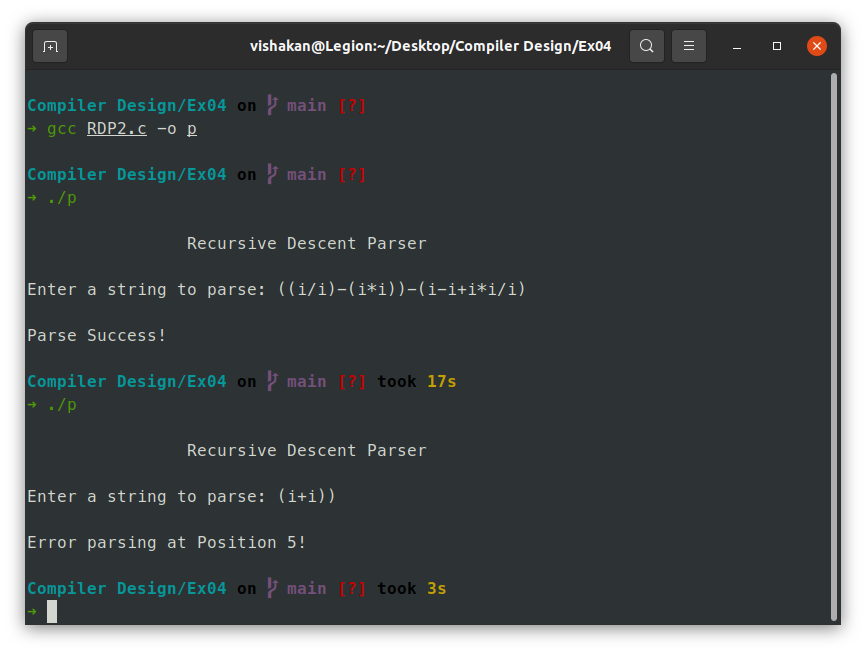
\includegraphics[scale= 0.5]{RDP2OP.png}
\end{figure}

%Learning Outcome
\newpage
\subsection*{\flushleft{Learning Outcome:}}
\begin{itemize}

\item I understood about the working of a \textbf{Recursive Descent Parser}.
\item I understood that Recursive Descent Parser, being a Top-Down Parser, does not work with Left-Recursive Grammars.
\item I was able to implement a working Recursive Descent Parser for a simple grammar.
\item I was able to extend the concept to implement a Recursive Descent Parser for a complicated grammar with more productions.
\item I refreshed my concepts with recursion \& return handling in functions with C.
\item I understood how to manually perform the Recursive Descent Parsing Process.
\end{itemize}


\end{document}